\begin{tcolorbox}[title=Example 1: The n-Queens Problem (1/2)]
\textbf{Exercise:}  
\\ The n-queens problem asks for a placement of $n$ queens on an n × n
chessboard so that no queen can attack another queen. This means that no two queens can be
placed in the same row, in the same column, or on the same diagonal. We display a solution
to the eight-queens problem below.

\centering
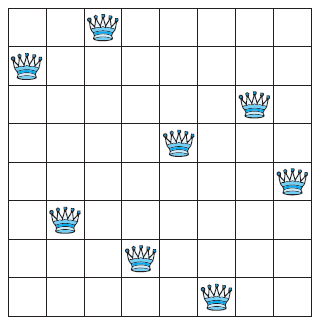
\includegraphics[width=0.3\linewidth]{chp1_3_propequiv/n_queens.png}

\raggedright
\textbf{Strategy:} \newline 
To model the n-queens problem as a satisfiability problem, we introduce $n^2$ variables, $p(i,j)$ for $i = 1,2, \ldots, n$ and $j = 1,2, \ldots, n$.
\newline For a given placement of a queens on the chessboard:
\begin{center}
$p(i, j)$ is \textbf{true} when there is a queen on the square in the i'th row and j'th column. \newline and \textbf{false} otherwise.
\end{center}
Note that squares $(i,j)$ and $(i', j')$ are on the same diagonal if either:
\begin{center}
$i+ i' = j+ j'$ \ \ or \ \ $i-i' = j - j'$    
\end{center}
\textbf{Implementing solution:} \newline
\textbf{Step 1:}
For no two of the $n$ queens to be in the same row, there must be one queen in each row. We
can show that there is one queen in each row by verifying that every row contains at least one
queen and that every row contains at most one queen. 
\begin{center}
$\bigvee_{j=1}^{n} p(i,j)$ asserts that
row $i$ contains at least one queen \newline
$Q_1 = \bigwedge_{i=1}^{n} \bigvee_{j=1}^{n} p(i,j)$ \textbf{asserts that every row contains at least one queen}
\end{center}
\textbf{Step 2:} For every row to include at most one queen, it must be the case that $p(i, j)$ and $p(k, j)$ are
not both true for integers $j$ and $k$ with $1 \leq j < k \leq n$. \newline
Observe that $\neg p(i,j) \lor \neg p(i,k)$ asserts that at least one of $\neg p(i,j)$ and $\neg p(i,k)$  is true, which means that at least one of $p(i, j)$ and $p(i, k)$ is false.
So, to check that there is: 
\begin{center}
$Q_2 = \bigwedge_{i=1}^n \bigwedge_{j=1}^{n-1} \bigwedge_{k=j+1}^{n} (\neg p(i,j) \lor \neg p(k,j)) $    \ \textbf{asserts at most one queen in each row}
\end{center}
\textbf{Step 3:} We have do the same, but for coloumns:
\begin{center}
$Q_3 = \bigwedge_{i=1}^n \bigwedge_{j=1}^{n-1} \bigwedge_{k=i+1}^{n} (\neg p(i,j) \lor \neg p(k,j)) $     \textbf{no column contains more than one queen}
\end{center}   
\end{tcolorbox}

\newpage
\begin{tcolorbox}[title=Example 1: The n-Queens Problem (2/2)]
\textbf{Step 4:} Now we consider the diagonals, and we have to make sure, that no diagonal contains two queens. We will first look at the main diagonal, which are characterized by having constant values of $i-j$. So we have to enforce that for all cells ($i,j$) there is no other queen on $(i+k, j+k)$, where $k$ increases along the diagonal:
\begin{center}
$Q_4 = \bigwedge_{i=1}^{n-1} \bigwedge_{j=1}^{n-1} \bigwedge_{k=1}^{min(n-i,n-j)} (\neg p(i,j) \lor \neg p(i+k,j+k)) $   \ \  \textbf{Main diagonal}
\end{center} 
\textbf{Step 5:} These anti-diagonals are characterized by constant values of $i+j$. So we have to enforce that for all cells ($i,j$) there is no other queen on $(i+k, j-k)$, where $k$ increases along the diagonal: 
\begin{center}
$Q_5 = \bigwedge_{i=1}^{n-1} \bigwedge_{j=2}^{n} \bigwedge_{k=1}^{min(n-i,j-1)} (\neg p(i,j) \lor \neg p(i+k,j-k)) $  \ \  \textbf{Anti-diagonal} 
\end{center} 
\textbf{Step 6:} Putting all this together, we find that the solutions of the n-queens problem are given
by the assignments of truth values to the variables $p(i,j) $ 
\begin{center}
$i=1,2,\ldots,n$  and $j=1,2,\ldots,n$ that make the following true
\end{center}
\begin{center}
$Q=Q_1 \land Q_2 \land Q_3 \land Q_4 \land Q_5$    
\end{center}{}
\end{tcolorbox}


\begin{tcolorbox}[title=Example 2: Sudoku puzzles (1/2)]
\textbf{Exercise:} \newline
Sudoku puzzles are constructed using a 9 × 9 grid made up of nine 3 × 3 subgrids, known as blocks \newline
For each puzzle, some of the 81 cells, called givens,
are assigned one of the numbers 1, 2,…, 9, and the other cells are blank. The puzzle is solved
by assigning a number to each blank cell so that every row, every column, and every one of the
nine 3 × 3 blocks contains each of the nine possible numbers.
\newline Note that instead of using a 9 × 9
grid, Sudoku puzzles can be based on $n^2 \times n^2$ grids, for any positive integer n, with the $n^2 \times n^2$ 
grid made up of $n^2$ $n \times n$  subgrids.
\newline \newline
\textbf{Strategy:} \newline 
To encode a Sudoku puzzle, let $p(i, j, n)$ denote the proposition that is true when the number
n is in the cell in the i'th row and j'th column. There are 9 × 9 × 9 = 729 such propositions, as i,
j, and n all range from 1 to 9. For example, for the puzzle in Figure 2, the number 6 is given as
the value in the fifth row and first column. Hence, we see that $p(5, 1, 6)$ is true, but $p(5, j, 6)$ is
false for $j = 2, 3,\ldots, 9$.
\newline 
\newline
Given a particular Sudoku puzzle, we begin by encoding each of the given values. Then,
we construct compound propositions that assert that every row contains every number, every
column contains every number, every 3 × 3 block contains every number, and each cell contains
no more than one number. \newline It follows, as the reader should verify, that the Sudoku puzzle is solved
by finding an assignment of truth values to the 729 propositions $p(i, j, n)$ with $i$, $j$, and $n$ each
ranging from 1 to 9 that makes the conjunction of all these compound propositions true. \newline After
listing these assertions, we will explain how to construct the assertion that every row contains
every integer from 1 to 9. \newline We will leave the construction of the other assertions that every
column contains every number and each of the nine 3 × 3 blocks contains every number to the
exercises
\end{tcolorbox}

\newpage
\begin{tcolorbox}[title=Example 2: Sudoku puzzles (2/2)]
\textbf{Solution:} \newline
\textbf{Step 1:} \newline
For each cell with a given value, we assert $p(i, j, n)$ when the cell in row $i$ and column $j$
has the given value $n$.
\newline \textbf{Step 2:} \newline
First, to \textbf{assert that row $i$ contains the number $n$}, we form
\begin{center}
$\bigvee_{j=1}^9 p(i,j,n)$    
\end{center}
\textbf{Step 3:}
\newline
To assert that\textbf{ row $i$ contains all $n$ numbers}, we form the conjunction of these disjunctions over all nine possible values of $n$, giving us
\begin{center}
$\bigwedge_{n=1}^9 \bigvee_{j=1}^9 p(i,j,n)$    
\end{center}
\textbf{Step 4:}
\newline
Finally, to \textbf{assert that every row contains  every number}, we take the conjunction
\begin{center}
$\bigwedge_{i=1}^9 \bigwedge_{n=1}^9 \bigvee_{j=1}^9 p(i,j,n)$    
\end{center}
\textbf{Step 5:}
\newline
(Exercises 71 and 72 ask for explanations of the assertions
that every column contains every number and that each of the nine 3 × 3 blocks contains
every number.)
\begin{center}
$\bigwedge_{j=1}^9 \bigwedge_{n=1}^9 \bigvee_{i=1}^9 p(i,j,n)$ \ \ \ \textbf{assert that every column contains every number}  \newline \newline
And that \textbf{assert that each of the nine 3 × 3 blocks contains every number;}
$\bigwedge_{r=0}^2 \bigwedge_{s=0}^2 \bigwedge_{n=1}^9 \bigvee_{i=1}^3 \bigvee_{j=1}^3 p(3r+i,3s+j,n)  $
\end{center}

\end{tcolorbox}




